\documentclass[11pt]{article}
\usepackage{icmlko}
\begin{document}

\title{조용히 죽어 있던 열 --- 서랍을 전수조사하니 절반이 안 꽂혀 있거나 고장 나 있었다}
\author{월드모델 실험실}
\date{노트 415 · 2026년 8월 2일}
\maketitle

\begin{abstract}
노트 413이 \texttt{grp} 하나로 판을 $+0.0029$ 올리면서 한 줄을 남겼다 ---
\emph{grp 가 이렇게 오래 안 쓰였다면 다른 것도 있다.} 축 모듈 열둘을 전부
지어 챔피언과 대조했다. 안 꽂힌 것: \texttt{seqaxes}(속편 여부, 7 도메인
$100\%$) · \texttt{popaxes}(팝업 전용 넷) · \texttt{mktaxes}/\texttt{mktmore}
(노트 412) · \texttt{creatoraxes}(중복, 노트 413) · \texttt{animeaxes} ·
\texttt{recaxes}(축 0).

\texttt{seqaxes} 를 관문에 올렸다. 노트 181이 지은 축이다 --- \emph{위키
수준$\leftrightarrow$라벨의 부호가 도메인마다 반대인 까닭이 속편이다}(애니
속편 $\rho{=}-0.28$ 대 신작 $+0.04$). 제목만 보면 아는 값이라 누수가 없다.

\begin{center}
\begin{tabular}{lrr}
\hline
짝 12뽑기 & 판 & 부호 \\
\hline
B $+$seq & $-0.0000$ & $7/12$ \\
\hline
\textbf{애니} & $\mathbf{+0.0103}$ & $\mathbf{12/12}$ \\
아이돌 (안 덮임) & $+0.0293$ & $12/12$ \\
\textbf{도서} (학습 80행) & $\mathbf{-0.0434}$ & $0/12$ \\
\hline
\end{tabular}
\end{center}

\textbf{판에서는 정확히 0 이다.} 미리 적어 둔 실패 조건이 걸렸다 ---
\emph{seq 가 이미 위키 축에 흡수돼 있으면 0 이다.} 그런데 도메인별로 보면
\textbf{축은 진단한 자리에서 정확히 일한다} --- 노트 181이 속편 효과를 잰
도메인이 애니이고, 애니가 $+0.0103 \cdot 12/12$ 로 오른다. 그것을 지우는
것은 \textbf{학습 80행짜리 도서}가 혼자 내는 $-0.0434$ 다.

그리고 노트 413의 놀라움이 \textbf{재현됐다} --- 덮인 도메인 평균
$-0.0057$ 대 \textbf{안 덮인 평균 $+0.0064$}.
\end{abstract}

\section{세 번째 팔이 아무 일도 안 했다}

\texttt{popaxes} 를 같이 얹은 팔 C 는 \textbf{열한 도메인 전부에서 B 와
소수점 넷째 자리까지 똑같이} 나왔다. 열둘 뽑기가 전부 같은 값일 확률은
없다 --- 자질 행렬이 안 바뀐 것이다.

열어 보니 \texttt{popaxes} 는 \textbf{75행}으로 지어져 있고 판의 팝업은
\textbf{89행}이다(노트 358이 등급 필터를 풀어 $75 \to 89$ 로 넓혔다).
\texttt{harness.load} 가 길이 불일치로 떨어뜨리고 중립 $0.5$ · 표시자 $0$ 을
채운다. 네 열의 \textbf{관측 표시자 평균이 정확히 $0.000$} 이다.

\textbf{노트 358 이후로 이 축 넷은 죽어 있었다.} 관문에 올리면 ``무해''로
보이는데 실은 \textbf{한 번도 안 재 본 것}이다. 사전 등록 ③(``단일 도메인
축은 판에 해롭다'')은 그래서 \textbf{시험되지 않았다} --- 그렇게 적는다.

\textbf{규약을 하나 더 만들고 코드에 넣었다}: \texttt{lab/loop.py} 의
\texttt{\_dead\_axes} 가 \textbf{표시자가 어디서도 1 이 아닌 축}을 실행
기록에 남긴다. 지금 챔피언은 죽은 축 0 이고, \texttt{popaxes} 를 얹으면
넷을 바로 짚는다. 거부권이 아니라 이름표다.

\section{판은 축을 재는 자로 무디다}

노트 412(시장팝업 $+0.0241$, 판 $+0.0005$) · 노트 413(판 $+0.0029$인데
\textbf{안 덮인} 쪽이 여섯 배) · 이번(애니 $+0.0103$, 판 $-0.0000$) 이
같은 모양이다. \textbf{축을 넣으면 이득이 한둘에 몰리고, 어느 도메인이
그것을 지울지는 미리 못 맞힌다.} 세 번 다 사전 등록이 도메인 쪽에서
틀렸다.

\begin{tabular}{lp{7.2cm}}
\hline
도서 & 학습 80행으로 판 무게 $163/3430$ 을 갖는다. 축을 넣을 때마다 이
도메인이 값을 정한다 \\
축을 도메인별로 켜고 끄기 & 애니엔 켜고 도서엔 끄면 둘 다 얻는다. 그런데
그 선택은 \textbf{라벨을 봐야} 하고 안 본 도메인엔 못 쓴다 --- 노트 409·410이
만난 벽 \\
popaxes 고치기 & 89행으로 다시 지으면 처음으로 재 볼 수 있다 \\
\hline
\end{tabular}

\begin{figure}[h]
\centering
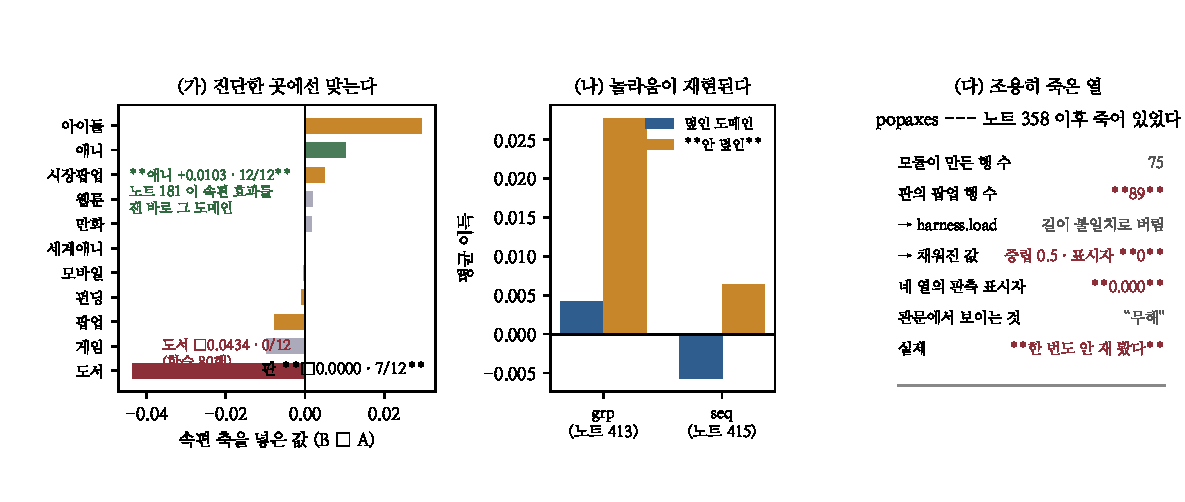
\includegraphics[width=\textwidth]{figs/fig415.pdf}
\caption{(가) 도메인별 --- 애니가 오르고 도서가 지운다. (나) 노트 413의
``안 덮인 쪽이 더 번다''가 재현된다. (다) \texttt{popaxes} 가 죽어 있던 경로.}
\end{figure}

\end{document}
